\documentclass{article}

\usepackage[
    backend=biber, % Use Biber for bibliography compilation.
    style=ieee, % Style for in-text citations.
    sorting=none, % References in the order they are cited.
    natbib=true % Enable natbib compatibility.
]{biblatex}
\usepackage{xcolor}
\definecolor{darkpurple}{RGB}{102, 0, 204}
\definecolor{darkerpurple}{RGB}{51, 0, 102}
\usepackage{hyperref}
\hypersetup{
    hidelinks=true,
    colorlinks=true,
    linkcolor=darkerpurple,    % internal links
    urlcolor=darkerpurple,     % external links
    citecolor=darkerpurple,     % citations
}
\usepackage{amsmath}
\usepackage{amssymb}
\usepackage{amsfonts}
\usepackage{geometry}
\usepackage{graphicx}
\usepackage{caption}
\usepackage[acronym]{glossaries}
\usepackage{comment}
\geometry{a4paper, margin=1in}

\addbibresource{references.bib} % Replace with your actual .bib filename

\glsdisablehyper


%===============================================================================

\newacronym[%
    longplural={blood vessels},%
    shortplural={BV},%
]{BV}{BV}{blood vessel}
\newacronym{AV}{A/V}{arteries and veins}
\newacronym{RR}{RR}{Recursive Refinement}
\newacronym{GAVE}{GAVE}{Generalized Analysis of Vessels in Eye}
% \newacronym{FOV}{FOV}{field of view}
\newacronym[
    longplural={regions of interest},%
    shortplural={ROIs},%
]
{ROI}{ROI}{region of interest}
\newacronym{HSV}{HSV}{hue, saturation, and value}
\newacronym{CLAHE}{CLAHE}{contrast limited adaptive histogram equalization}
\newacronym{CGCELIN}{CGCELIN}{channel-wise global contrast enhancement and local intensity normalization}
\newacronym{GT}{GT}{ground truth}
\newacronym{BCE}{BCE}{binary cross-entropy}
\newacronym{TTA}{TTA}{test-time augmentation}

%===============================================================================


\makeglossaries



% Document
\begin{document}

\title{\bfseries GAVE Challenge Team Technical Report}
\author{%
    Team Name: \texttt{R2-V2} \\
    Team Members: José Morano\thanks{%
        Christian Doppler Laboratory for Artificial Intelligence in Retina, Institute of Artificial Intelligence, Medical University of Vienna, Vienna, Austria. Email: \texttt{jose.moranosanchez@meduniwien.ac.at}%
    }
}
 \date{\today}
\maketitle

\begin{abstract}
    This document presents the technical report for the \texttt{R2-V2} team participating in the \gls{GAVE} Challenge.
    The report details our approach, methodologies, and experimental configurations employed in addressing the challenge Tasks 1 and 2, which involve the segmentation of blood vessels and their classification into arteries and veins in retinal images.
    No work was done for Task 3, so it is not included in this report.
\end{abstract}

%===============================================================================
%===============================================================================
%===============================================================================
\section{Proposed Method}


%===============================================================================
%===============================================================================
\subsection{Model Framework}

\begin{figure}[h]
    \centering
    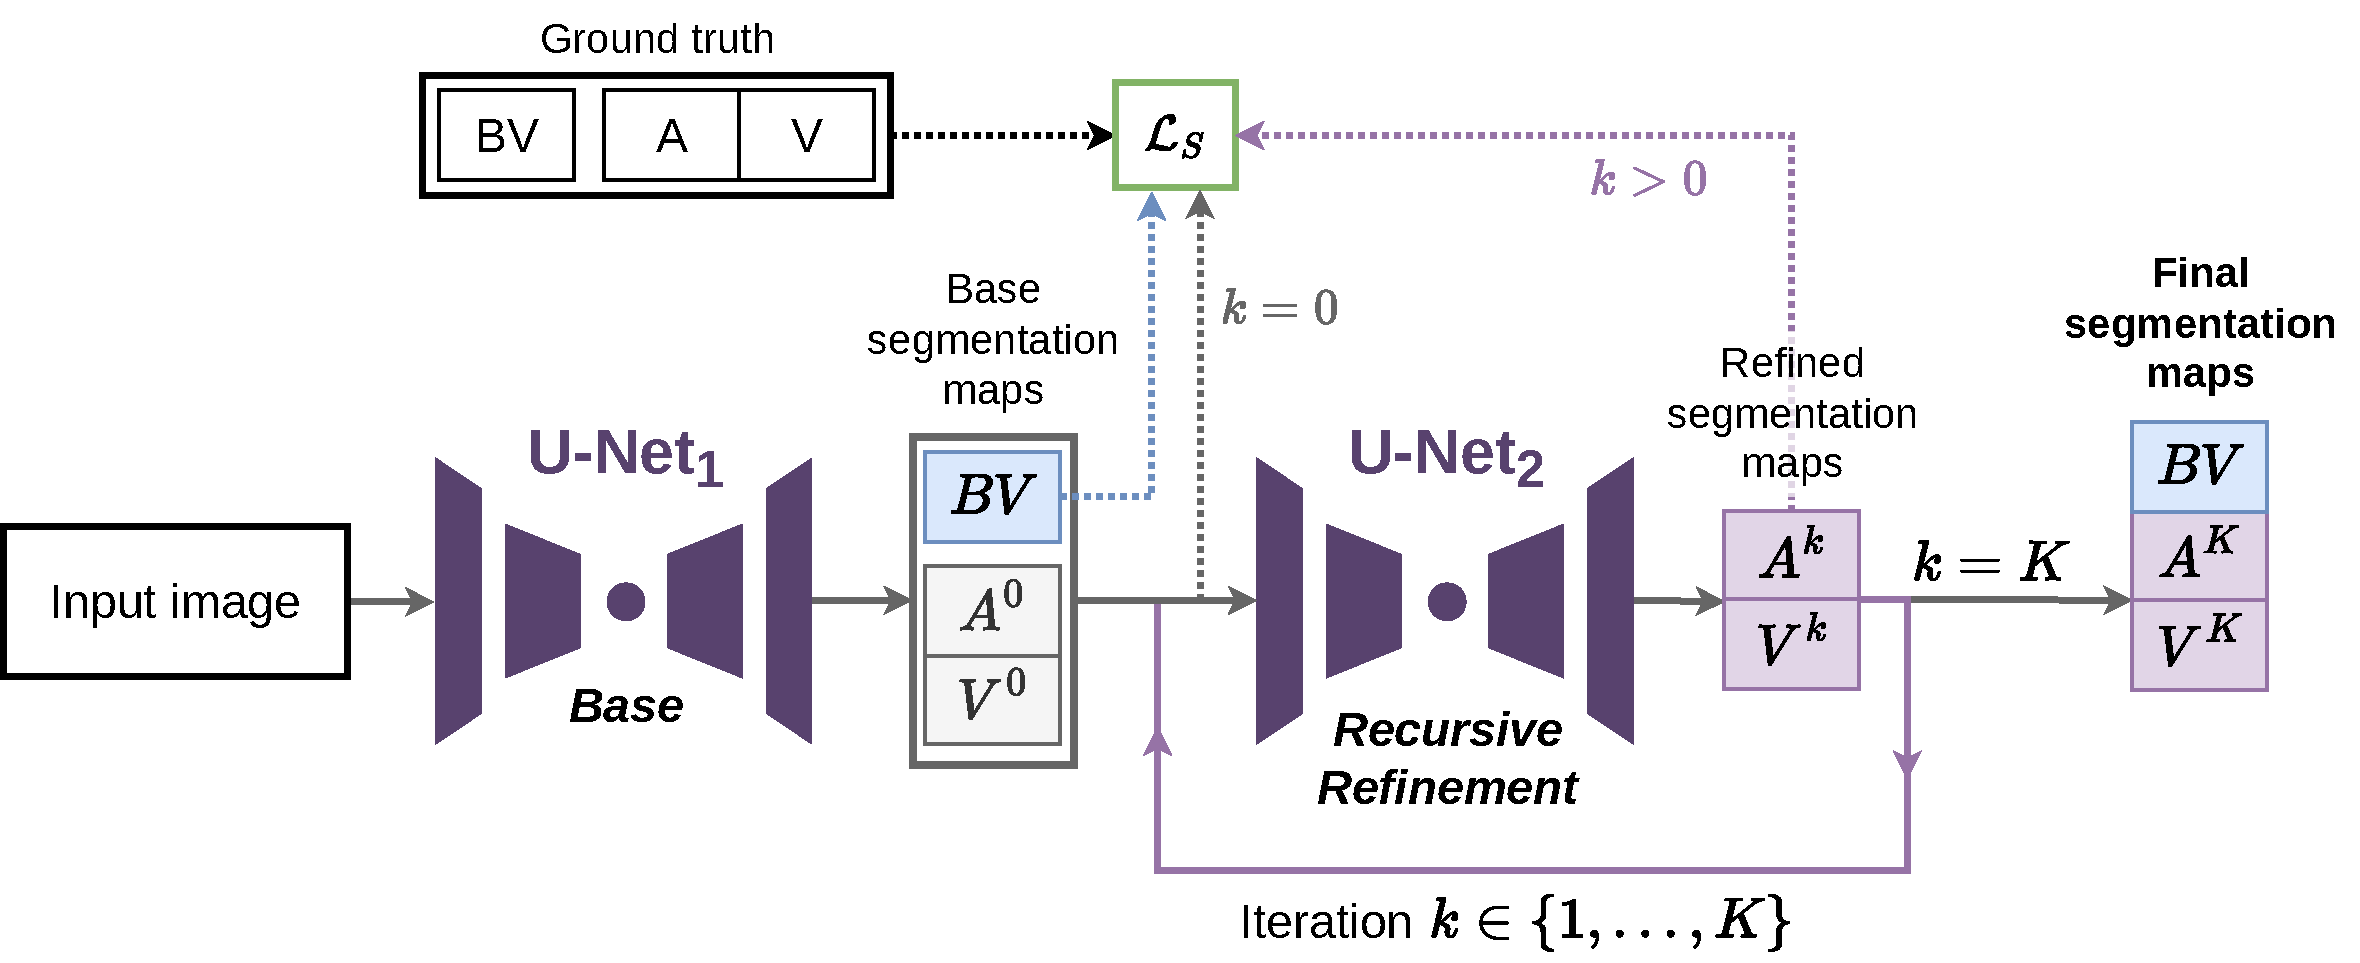
\includegraphics[width=0.85\textwidth]{figs/method.pdf}
    \caption{Proposed method, based on~\cite{morano2024rrwnet}.}
    \label{fig:rrwnet_architecture}
\end{figure}

\begin{figure}[h]
    \centering
    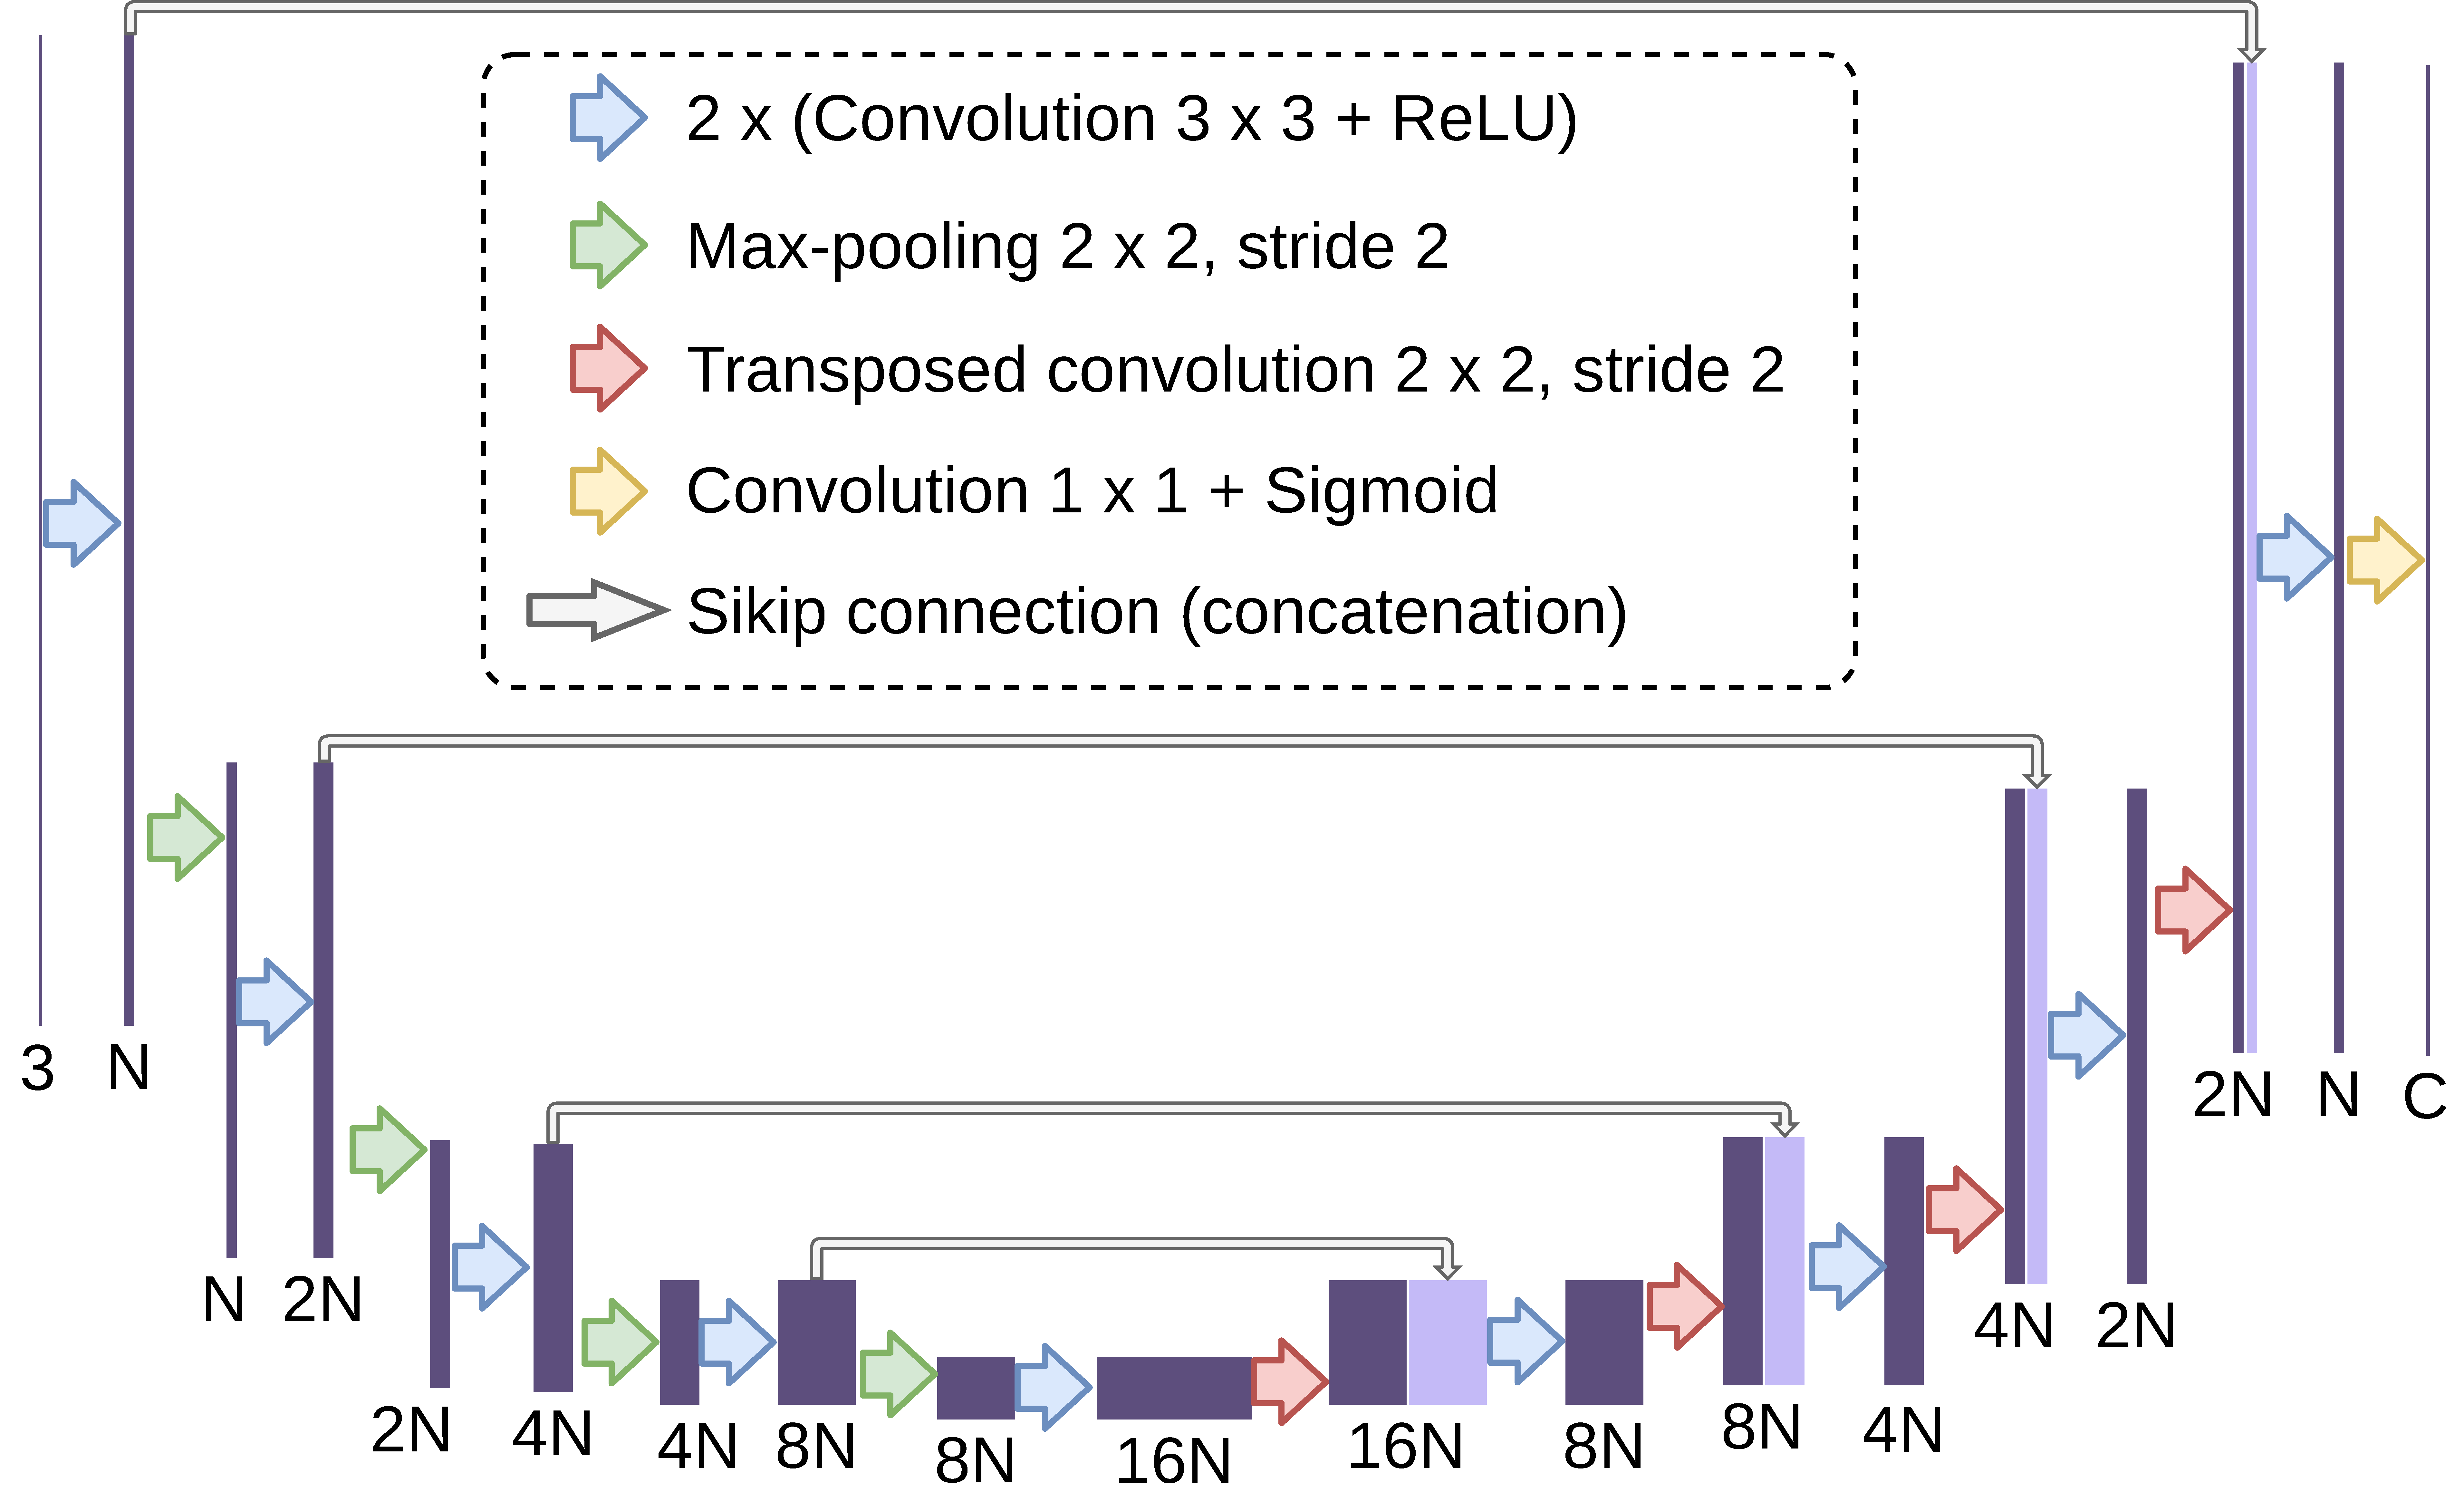
\includegraphics[width=0.6\textwidth]{figs/unet.pdf}
    \caption{U-Net architecture~\cite{ronneberger2015unet}.}
    \label{fig:rrwnet_block}
\end{figure}


%===============================================================================
%===============================================================================
\subsection{Structure Detail Description}

Our approach is based on the RRWNet architecture~\cite{morano2024rrwnet}, which is depicted in Figure~\ref{fig:rrwnet_architecture}.
The architecture consists of two main components: the Base segmentation module and the \gls{RR} module.
Both components are based on a standard U-Net architecture~\cite{ronneberger2015unet}, shown in Figure~\ref{fig:rrwnet_block}, only adapting the number of input and output channels.

The Base segmentation module generates an initial segmentation of \glspl{BV}, arteries, and veins from the input image.
Then, the \gls{RR} module refines the initial \gls{AV} segmentation in a recursive and iterative manner, improving the segmentation quality.
The final output of the model is the combination of the initial \gls{BV} segmentation from the Base segmentation module and the refined \gls{AV} segmentation from the \gls{RR} module.

%===============================================================================
%===============================================================================
\subsection{Input/Output (Data Flow)}

Let $\mathbf{x} \in \mathbb{R}^{3 \times H \times W}$ be the input RGB color fundus image, where $H$ and $W$ are its height and width, respectively.
To obtain the final prediction $\mathbf{\hat{y}} \in \mathbb{R}^{3 \times H \times W}$, we apply the network $f(\mathbf{x}, \theta, K)$ to the input image $\mathbf{x}$, where $\theta$ represents the learnable parameters of the network and $K$ denotes the number of iterations performed by the \gls{RR} subnetwork.
Thus, the output of the network $\mathbf{\hat{y}}_k$ at an arbitrary iteration $k$ can be defined as
%
\begin{equation}\label{eq:network}
    \small
    \begin{aligned}
        \mathbf{\hat{y}}_k &= f(\mathbf{x}, \theta, k) \\
        &= \begin{cases}
            f_R(f(\mathbf{x}, \theta, k-1), \theta^R)_\text{a,v} \oplus f_B(\mathbf{x}, \theta^B)_\text{bv}, & k > 0 \\
            f_B(\mathbf{x}, \theta^B), & k = 0
        \end{cases}
    \end{aligned}
\end{equation}
%
where
$f_B$ and $f_R$ represent the Base and \gls{RR} subnetworks with parameters $\theta^B$ and $\theta^R$, respectively;
the subscripts a, v, and bv denote the channels corresponding to the segmentation maps of the different structures;
and $\oplus$ denotes the concatenation operation in the channel dimension.



%===============================================================================
%===============================================================================
%===============================================================================
\section{Experiment Configuration}


%===============================================================================
%===============================================================================
\subsection{Datasets}

For training the model, we used the training set provided by the \gls{GAVE} Challenge along with the following public datasets: RITE~\cite{hu2013rite,staal2004ridge}, HRF~\cite{budai2013robust,chen2022twgan}, and LES-AV~\cite{orlando2018lesav}, Fundus-AVSeg~\cite{deng2025fundusavseg}, AFIO~\cite{afio2020}, and DualModal2019~\cite{dualmodal2019}.
All these datasets provide annotations for arteries and veins as well as for the \glspl{ROI} (i.e., the retinal area visible in the image).
The combination of these datasets provides a diverse set of 386 color fundus images.

%===============================================================================
%===============================================================================
\subsection{Datasets Split Method}

For the development of the model, we randomly split the combined dataset into training, validation, and test sets (70\%, 15\%, and 15\% of the total data, respectively).
However, for the preliminary submission, we trained the model using all the available data.
In this way, the final models were trained using the 386 images.

%===============================================================================
%===============================================================================
\subsection{Data Augmentation}

To enhance the diversity of the training data and improve the generalization of the model, we applied strong data augmentation.
The full list of augmentations is detailed below.
In each case, the distribution from which the augmentation parameters are sampled (if applicable) is indicated, along with the probability $p$ of applying the augmentation operation.

\begin{itemize}
    \item Horizontal and vertical flips ($p=0.5$ each).
    \item Random rotations with angle $\theta \sim \mathcal{U}(-180^\circ, 180^\circ)$ ($p=1$).
    \item Random scaling with factor $\alpha \sim \mathcal{U}(0.7, 1.4)$ ($p=1$).
    \item Random shearing with angle $\gamma \sim \mathcal{U}(-25^\circ, 25^\circ)$ ($p=1$).
    \item Random \gls{HSV} color jittering ($p=1$):
        \begin{itemize}
            \item $\Delta\text{H}  \sim \mathcal{U}(-0.02, 0.02)$.
            \item $\Delta\text{S} \sim \mathcal{U}(-0.2, 0.2)$.
            \item $\Delta\text{V} \sim \mathcal{U}(-0.2, 0.2)$.
            \item For H and V, there is also a multiplicative factor $m \sim \mathcal{U}(0.8, 1.2)$.
        \end{itemize}
    \item Random cutout ($p=0.8$):
        \begin{itemize}
            \item 16 patches of size $0.04\times0.04$ of the image size.
            \item Top left coordinates $(i,j)$ sampled uniformly across the image, so that $i \sim \mathcal{U}(0, W)$ and $j \sim \mathcal{U}(0, H)$, where $W$ and $H$ are the width and height of the image, respectively.
            \item The value inside each patch is sampled from $\mathcal{U}(0.4, 0.6)$.
        \end{itemize}
\end{itemize}


For inference, we use \gls{TTA} with horizontal and vertical flips as well as 90-degree rotations, resulting in a total of 8 different augmentations (including the original image).


%===============================================================================
%===============================================================================
\subsection{Preprocessing}

As preprocessing, we applied \gls{CGCELIN} (as proposed in~\cite{morano2021simultaneous}) followed by \gls{CLAHE}~\cite{zuiderveld1994clahe}.
In particular, \gls{CGCELIN} is defined as follows:

\begin{align*}
I_{\mathrm{norm}}^C = \sigma_0  \frac{I^C-{I^C_l}}{\sigma_{I^C-{I^C_l}}} \ ,
\end{align*}

where $I_{\mathrm{norm}}^C$ is the normalized channel $C$, $I^C$ is the channel $C$ of the original input image, $I_l^C$ is the low-pass filtered channel $C$ and $\sigma_{I^C-I_l^C}$ is the global standard deviation of the channel resulting from the subtraction of the low-pass filtered channel $I_l^C$ to the original channel $I^C$.

As in~\cite{morano2021simultaneous}, we use $\sigma_0 = 1$, with a Gaussian filter with zero mean and standard deviation $\sigma = 10$.
For training, the input images were cropped to the \gls{ROI} using the provided masks and resized to a fixed width of 1408 pixels, maintaining the original aspect ratio.
For inference in the \gls{GAVE} validation set, no resizing nor cropping was applied, and the images were processed at their original resolution.


%===============================================================================
%===============================================================================
\subsection{Training Strategy}

%===============================================================================
\subsubsection*{Loss Function}

To train the network, we build on the loss function proposed in~\cite{morano2024rrwnet}.
Specifically, the total loss $\mathcal{L}$ combines the segmentation errors from each iteration $k \in \{0,...,K\}$ with different weights.
This loss is defined as:
%
\begin{equation}\label{eq:loss}
    \mathcal{L}\left(\mathbf{\hat{y}},\mathbf{y}\right) ~=~ \sum_{k=0}^{K} w_k \mathcal{L}_\text{S}\left(\mathbf{\hat{y}}_k,\mathbf{y}\right) \ ,
\end{equation}
%
where
$w_k$ is the weight of the loss at iteration $k$,
$\mathbf{\hat{y}}_k$ is the output of the network at iteration $k$ (see Eq.~\ref{eq:network}),
$\mathbf{y}$ is the \gls{GT},
% Similarly, the ground truth (GT) $\mathbf{y} \in \mathbb{R}^{3 \times H \times W}$ also has three channels, corresponding to the manual segmentation maps of arteries ($\mathbf{y}^A$), veins ($\mathbf{y}^V$), and vessels ($\mathbf{y}^{BV}$). 
and $\mathcal{L}_\text{S}$ is the base segmentation loss function.
The weighting scheme is the same as in \cite{morano2024rrwnet}, giving a higher weight to the error of the first iteration ($k=0$), which solely relies on the Base subnetwork.
Specifically, the weight $w_k$ at iteration $k$ is defined as
%
\begin{equation}\label{eq:weights}
    w_k =
    \begin{cases}
        1, & k = 0 \\
        \frac{1}{Z} \sum_{k=1}^{K} k \mathcal{L}_\text{S}\left(\mathbf{\hat{y}}_k,\mathbf{y}\right), & k > 0
    \end{cases}
\end{equation}
%
with the normalization factor $Z = \sum_{k=1}^{K} k = \frac{K(K+1)}{2}$.

While the general formulation is the same as in~\cite{morano2024rrwnet}, the specific definition of $\mathcal{L}_\text{S}$ is different, as explained next.
In particular, we adapt the loss function to focus on multiple aspects of the segmentation task, including vessel presence, \gls{AV} discrimination, \gls{AV} mutual exclusion, crossing identification, and background consistency.
Formally, the total base loss function $\mathcal{L}_\text{S}$ can be defined as:

\begin{equation}
\mathcal{L}_\text{S} =
    \lambda_{\text{bv}} \cdot \mathcal{L}_{\text{bv}}
    + \lambda_{\text{av}} \cdot \mathcal{L}_{\text{av}}
    + \lambda_{\text{mx}} \cdot \mathcal{L}_{\text{mx}}
    + \lambda_{\text{cr}} \cdot \mathcal{L}_{\text{cr}}
    + \lambda_{\text{bg}} \cdot \mathcal{L}_{\text{bg}} \ ,
\end{equation}
where each $\mathcal{L}_{(\cdot)}$ component corresponds to a specific aspect of the segmentation task, and $\lambda_{(\cdot)}$ are the corresponding weights.

% In most cases, we use \gls{BCE} as the function to ultimately compare the ground truth and the prediction for each case.
The definition of each component is shown below.
However, we will first introduce some notation to facilitate their explanation.
Since the components operate on specific structure predictions and regions of the image, we use subscripts in the predicted and \gls{GT} variables ($\hat{\textbf{y}}$ and $\textbf{y}$, respectively) to indicate the selected channel: a: artery, v: vein, bv: blood vessel (artery + vein).
Similarly, the superscripts are used to indicate the selected region (pixels) of the image: a: arteries, v: veins, bv: blood vessels (artery + vein), bg: background, cr: crossings, roi: region of interest, and a$\vee$v: arteries or veins (i.e., bv excluding crossings).
Moreover, $\odot$ denotes the element-wise multiplication, $\mathbf{0}$ and $\mathbf{1}$ are matrices of zeros and ones with the same size as the corresponding prediction, respectively, and $\text{avg}(\cdot)$ denotes the average value of all elements in the matrix.
With this notation, the different components of the loss function are defined as follows:

\begin{itemize}
    \item \textbf{Vessel Presence Loss}:
        \begin{equation}
        \mathcal{L}_{\text{bv}} = \text{BCE}(\hat{\textbf{y}}^\text{roi}_\text{bv}, \textbf{y}^\text{roi}_\text{bv})
        \end{equation}

    \item \textbf{Artery/Vein Discrimination Loss}:
        \begin{equation}
        \mathcal{L}_{\text{av}} = \text{BCE}(\hat{\textbf{y}}^\text{bv}_\text{a}, \textbf{y}^\text{bv}_\text{a}) + \text{BCE}(\hat{\textbf{y}}^\text{bv}_\text{v}, \textbf{y}^\text{bv}_\text{v})
        \end{equation}

    \item \textbf{Mutual Exclusion Loss}:
        \begin{equation}
        % \mathcal{L}_{\text{mx}} = \frac{1}{N_{\text{a}\vee\text{v}}} \sum_{\mathcal{M}_{\text{a}\vee\text{v}}} \hat{\textbf{y}}_\text{a}^{\text{a}\vee\text{v}} \odot \hat{\textbf{y}}_\text{v}^{\text{a}\vee\text{v}}
        \mathcal{L}_{\text{mx}} =  \text{avg}\left(\hat{\textbf{y}}_\text{a}^{\text{a}\vee\text{v}} \odot \hat{\textbf{y}}_\text{v}^{\text{a}\vee\text{v}}\right)
        \end{equation}

    \item \textbf{Crossings Handling Loss}:
        \begin{equation}
        \mathcal{L}_{\text{cr}} = \text{BCE}\left(\frac{\hat{\textbf{y}}^\text{cr}_\text{a} + \hat{\textbf{y}}^\text{cr}_\text{v}}{2}, \textbf{1}\right)
        \end{equation}

    \item \textbf{Background Consistency Loss}:
    \begin{equation}
        \mathcal{L}_{\text{bg}} = \text{BCE}(\hat{\textbf{y}}_\text{a}^{\text{bg}}, \mathbf{0}) + \text{BCE}(\hat{\textbf{y}}_\text{v}^{\text{bg}}, \mathbf{0})
    \end{equation}
\end{itemize}


%===============================================================================
\subsubsection*{Optimization Details}

The models were trained using the Adam~\cite{kingma2015adam} optimizer with a learning rate of $1e-4$ and decay rates $\beta_1 = 0.9$ and $\beta_2 = 0.999$, as in~\cite{kingma2015adam}.
The batch size used is 1, to allow for variable input sizes.
The final models were trained for 200\,000 iterations ($\approx$ 518 epochs).



%===============================================================================
%===============================================================================
\subsection{Model Selection and Postprocessing}

For the preliminary submission, we trained two separate models:
$f_\text{BV}$, which focuses on segmenting \glspl{BV} and takes as input both the preprocessed and the original images (6 channels),
and $f_\text{AV}$, which focuses on classifying arteries and veins and takes as input only the preprocessed image (3 channels).
Both models use $K=6$ iterations in the \gls{RR} module, and are trained using the same loss function.
However, they differ in the specific weights used for each component of the loss function, in order to specialize each model for its specific task.

For training $f_\text{BV}$, the idea was to adjust the weights to put more emphasis on the discrimination between background and vessels.
For this reason, the weights of $\lambda_{\text{bv}}$, $\lambda_{\text{av}}$, and $\lambda_{\text{bg}}$ were set proportionally to the number of pixels belonging to the \gls{ROI} of each loss component scaled by some factors.
In particular, we use factors of 1.0, 2.0, and 0.5 for $\lambda_{\text{bv}}$, $\lambda_{\text{av}}$, and $\lambda_{\text{bg}}$, respectively.
Differently, the weights for the other two components, $\lambda_{\text{mx}}$ and $\lambda_{\text{cr}}$, are fixed to 0.5 and 0.2, respectively.
Formally, the weights for this model can be defined as follows:
\begin{equation}
    \lambda_{\text{bv}} = \frac{N_{\text{bv}}}{N_{\text{roi}}}, \quad
    \lambda_{\text{av}} = 2 \cdot \frac{N_{\text{a}\vee\text{v}}}{N_{\text{roi}}}, \quad
    \lambda_{\text{bg}} = 0.5 \cdot \frac{N_{\text{bg}}}{N_{\text{roi}}} , \quad
    \lambda_{\text{mx}} = 0.5, \quad
    \lambda_{\text{cr}} = 0.2 ,
\end{equation}
where $N$ denotes the number of pixels in the corresponding region, which is indicated by the subscript.
As can be seen, the higher weight is given to the background consistency loss (since around 80-90\% of the pixels belong to the background), followed the vessel presence loss.

On the other hand, for training $f_\text{AV}$, we set empirically the weights to the following values, in order to focus more on the \gls{AV} discrimination:

\begin{equation}
\lambda_{\text{vessel}} = 1.0, \quad
\lambda_{\text{av}} = 2.0, \quad
\lambda_{\text{bg}} = 0.5, \quad
\lambda_{\text{mx}} = 0.5, \quad
\lambda_{\text{cr}} = 0.5
\end{equation}

In this way, the highest weight is given to the \gls{AV} discrimination loss.

The final segmentation was obtained by combining the \gls{BV} segmentation from $f_\text{BV}$ and the \gls{AV} segmentation from $f_\text{AV}$.
However, before combining them, we apply a postprocessing step to improve the sensitivity of the \gls{BV} segmentation.
In particular, we set the segmented \glspl{BV} to include all the pixels classified as \glspl{BV}, arteries, or veins.
This is done by applying the following operation:
\begin{equation}
    \hat{\mathbf{y}}_\text{bv} = \max(\hat{\mathbf{y}}_\text{bv}, \text{clip}(\hat{\mathbf{y}}_\text{a} + \hat{\mathbf{y}}_\text{v}, 0, 1)) \ ,
\end{equation}
where $\hat{\mathbf{y}}_\text{bv}$, $\hat{\mathbf{y}}_\text{a}$, and $\hat{\mathbf{y}}_\text{v}$ are the predicted \gls{BV}, artery, and vein maps, respectively, $\max(\cdot, \cdot)$ is the element-wise maximum operation, and $\text{clip}(\cdot, 0, 1)$ limits the values to the range [0, 1].
No postprocessing is applied to the output segmentation maps of arteries and veins coming from the \gls{AV} model, except for setting to zero the pixels outside the \gls{ROI} using the provided masks, which is done for all the maps.

Consequently, the final output of the model is given by the concatenation of the \gls{BV} map from the \gls{BV} model and the artery and vein maps from the \gls{AV} model:
\begin{equation}
    \hat{\mathbf{y}} = \left(\hat{\mathbf{y}}_\text{bv} \oplus \hat{\mathbf{y}}_\text{a,v}\right) \odot \mathbf{m}_\text{roi} \ ,
\end{equation}
where $\hat{\mathbf{y}}_\text{bv}$ is the postprocessed \gls{BV} map from $f_\text{BV}$, $\hat{\mathbf{y}}_\text{a,v}$ are the artery and vein maps from $f_\text{AV}$, and $\mathbf{m}_\text{roi}$ is the binary mask of the \gls{ROI}.


%===============================================================================
%===============================================================================
\subsection{Technical Stack}

The implementation was done using Python 3.12, PyTorch 2.2\footnote{\url{https://pytorch.org/} [Accessed: Aug. 25, 2025]}, torchvision 0.17\footnote{\url{https://pytorch.org/vision/} [Accessed: Aug. 25, 2025]}, CUDA 12.1\footnote{\url{https://developer.nvidia.com/cuda-toolkit} [Accessed: Aug. 25, 2025]}, NumPy 1.26\footnote{\url{https://numpy.org/} [Accessed: Aug. 25, 2025]}, scikit-image 0.22\footnote{\url{https://scikit-image.org/} [Accessed: Aug. 25, 2025]}, and scipy 1.12\footnote{\url{https://scipy.org/} [Accessed: Aug. 25, 2025]}.
The training was performed using a NVIDIA A100 GPU with 80 GB of memory.


%===============================================================================
%===============================================================================
%===============================================================================
\section{GitHub}

The inference code for the proposed method is publicly available at \url{https://github.com/j-morano/R2-V2_materials}.


%===============================================================================
%===============================================================================
%===============================================================================
\printbibliography[title={\refname},heading=bibintoc]

\end{document}
